\documentclass[11pt,letterpaper,leqno]{amsart}
\usepackage[latin1]{inputenc}  % Unixin merkist?
\usepackage[T1]{fontenc}       % kirjaimet, joissa aksentteja (skandit)


\usepackage{amsfonts}         
\usepackage{amsmath}
\usepackage{amssymb}
\usepackage{amsthm}
\usepackage{ae,aecompl,amsbsy}
\usepackage{epsf}
\usepackage{graphics}
\usepackage{ucs}
\usepackage[pdftex]{graphicx}
\usepackage{amsaddr}
%\usepackage[foot]{amsaddr}


\usepackage{color}
\usepackage{verbatim}
\usepackage{algorithm}
\usepackage{algorithmic}
\usepackage{caption}
\usepackage{subcaption}

%bibligraphy
\usepackage[comma,sort]{natbib}
\usepackage{hyperref} 

\newcommand{\R}{\mathbb{R}}
\newcommand{\C}{\mathbb{C}}
\newcommand{\Q}{\mathbb{Q}}
\newcommand{\N}{\mathbb{N}}
\newcommand{\Z}{\mathbb{Z}}

\newcommand{\divergence}{\operatorname{div}}
\DeclareMathOperator*\argmin{argmin}

\newcommand{\TODO}[1]{\textcolor{red}{{\sc Todo:} #1}}


\newtheorem{definition}[equation]{Definition}
\newtheorem{proposition}[equation]{Proposition}
\newtheorem{assumption}[equation]{Assumption}
\usepackage{lineno}


\numberwithin{equation}{section}
\graphicspath{ {figures/} }

\title{Analytical results and physical understanding}
\author{Team C}

                               
\begin{document}

%\linenumbers
\maketitle
\thispagestyle{empty}

\bibliographystyle{plainnat}


\normalsize

\vspace{0.4cm}


\section{Uniform electric field illuminating a sphere in a uniform earth (analytic solution, reference)}



Let consider a  resistive uniform half-space, of conductivity $\sigma_1$enclosing a conductive sphere $\sigma_2$. Let assume a uniform, unidirectional static electric field $E_0$ going through this half-space.

\begin{figure}[h]
\caption{Uniform electric field illuminating a sphere in a uniform earth}
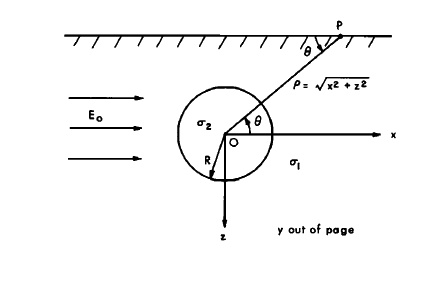
\includegraphics[scale=0.7]{ElectroStaticSphere.png}
\end{figure}

\section{Maxwell equations}

In this case, we need:

$\nabla \times E =0$ \quad,so \quad $E=-\nabla V$

$J=\sigma E$

The primary field $E_0$ can then be expressed by:

${E^p}_0=-\frac{dV^p}{dx}$

Assuming a primary potential null at the origin:

$V^p=E_0x=E_0 r cos\theta$

As [...], the anomalous or secondary field is expressed as:

$V^s=(A r + B r^{-2}) cos\theta$

\vspace{0.4cm}

 \vspace{0.4cm}



In this case, we need:

\begin{equation}
\begin{aligned}
\nabla \times E =0\\
J=\sigma E.
\end{aligned}
\end{equation}
The first equation gives $E=-\nabla V$.


The primary field $E_0$ can then be expressed by:
\begin{equation}
{E^p}_0=-\frac{dV^p}{dx}.
\end{equation}
Assuming a primary potential null at the origin:

 \begin{equation}
V^p=E_0x=E_0 r \cos\theta.
\end{equation}



As the primary potential respects $\nabla^2 V=0 $, as only a dependence in $x$ direction, the anomalous or secondary field can be expressed as (using spherical coordinates):

\begin{equation}
\begin{aligned}
V^s=(A r + B r^{-2}) \cos\theta.
\end{aligned}
\end{equation}


If we assume finite  values of the potential everywhere, we can divide the anomalous potential in two domain:


\begin{equation}
\begin{aligned}
&V^s_e=B r^{-2} \cos\theta  & \text{ if } r>R, \\
&V^s_i=A r \cos\theta & \text{ if }  r<R.
\end{aligned}
\end{equation}

 %\vspace{0.4cm}



The total external potential is then:

\begin{equation} 
V_e= V^s_e + {V^p} = (-E_0 r + B r^{-2}) \cos \theta.
\end{equation}

On the surface of the sphere, both the normal current density and potential have to be continuous across the interface.

 \vspace{0.4cm}


Using the continuity of current density, we got:
\begin{equation}
\begin{aligned}
\sigma_1 E_e & = \sigma_2 E_i \\
\sigma_1 \frac{dV_e}{dr} & = \sigma_2 \frac{dV_e}{dr}. \\
\end{aligned}
\end{equation}

%what's with this? Is something missing?
\begin{equation}\label{equ1}
2 \sigma_1 B R^{-3} + \sigma_1 E_0 = - \sigma_2 A
\end{equation}


Using the continuity of potential, we got:
\begin{equation}\label{equ2}
\begin{aligned}
{V_e}={V^s_i}.\\
-E_0 R + B R^{-2} = A R.\\
\end{aligned}
\end{equation}

From equations \ref{equ1} and \ref{equ2}, we get:

\begin{equation}
\begin{aligned}
A & =-\frac{3 \sigma_1}{\sigma_2 + 2\sigma_1} E_0 \\
B & =E_0 R^3 \frac{\sigma_2-\sigma1}{\sigma_2+2\sigma_1}. 
\end{aligned}
 \end{equation}

 \vspace{0.4cm}


\begin{figure}[h]
\caption{Induced Dipole moment P in a sphere in a uniform earth}
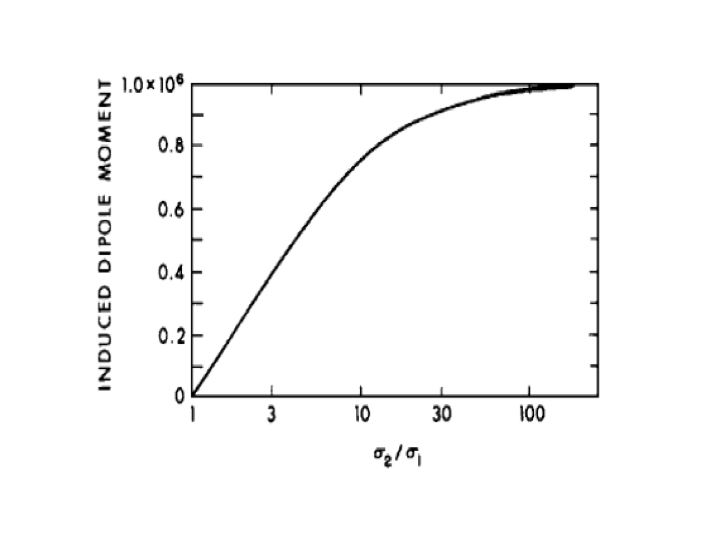
\includegraphics[scale=0.4]{SphereInducedDipoleMoment.png}
\label{Induced Dipole}
\end{figure}



\begin{figure}[h]
\caption{Anomalous field of a sphere in a uniform earth illuminated by an uniform electric field}
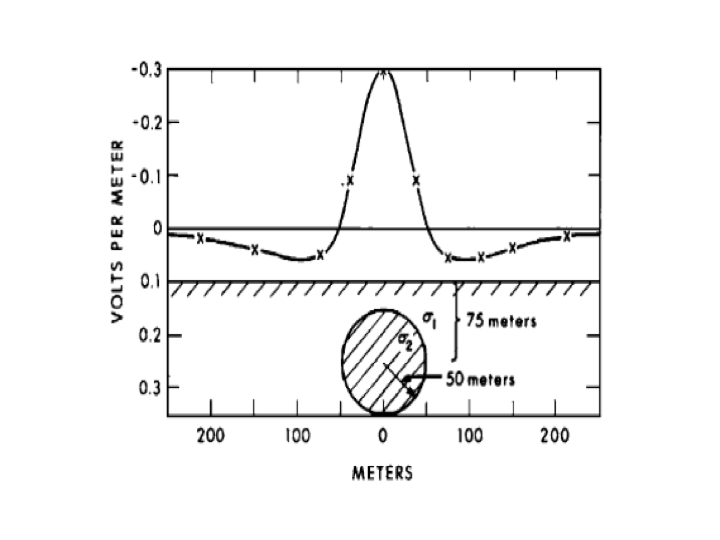
\includegraphics[scale=0.4]{SphereAnomlousField.png}
\label{Anomalous Field}
\end{figure}

And the anomalous electric field is:


\begin{equation}
\mathbf{E_s=-\nabla{V^s}_e=E_0 R^3 \frac{\sigma_2-\sigma_1}{\sigma_2 - 2\sigma_1} \frac{(2x^2-y^2-z^2)\mathbf{u}_x + 3xy \mathbf{u}_y + 3xz \mathbf{u}_z}{r^5}}. 
\end{equation}


\section{Continuity of current and charge accumulation}
We assume to be here in a steady state with direct current.
The current entering a cylinder through an interface as in figure \ref{Normal J continuous} consists both in tangential and normal components. 

\begin{figure}[h]
\caption{Uniform electric field illuminating a sphere in a uniform earth}
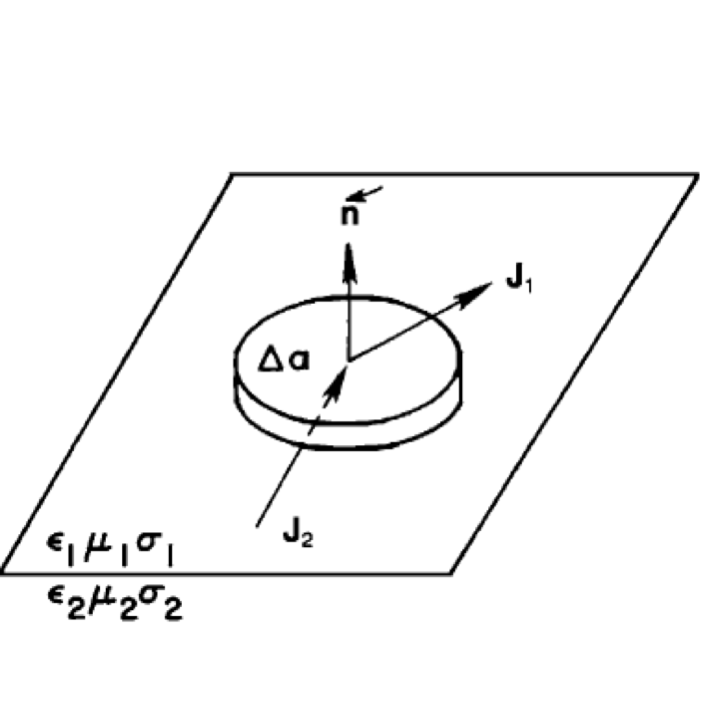
\includegraphics[scale=0.2]{Jcontinuous.png}
\label{Normal J continuous}
\end{figure}

As the cylinder height is collapsed to zero, we can write the normal component as:
\begin{equation}
I=J_1 \cdot \mathbf{n} \Delta a,
\text{or as}
I=J_2 \cdot \mathbf{n} \Delta a.
\end{equation}

Note: Otherwise in steady state we would have an infinite built up of charges at the interface. 
Then 
\begin{equation} 
J_2 \cdot \mathbf{n} = J_1 \cdot \mathbf{n},
 \end{equation}
so we have 
\begin{equation}
\mathbf{J_1^n=J_2^n}.
\end{equation}


Note: This is only true in a direct current case in a steady state. It appears to be satisfactory up to $10^5$ Hz, as long as displacement currents can be considered negligible.


\section{Charges, Coulomb's law and potentials.}

Electric charge produces an electric potential: the Coulomb's electrostatic potential is
\begin{equation}
V(r) = \frac{1}{4\pi\epsilon_0}\frac{Q}{r}.
\end{equation}



\section{Anomalous currents and electric fields}

Anomalous current density is defined as 
\begin{equation}
\mathbf{J}_a = \sigma_a\mathbf{E}.
\end{equation}


Here $\mathbf{E}$ is total electric field and $\sigma_a$ is the difference between wholespace conductivity $\sigma_1$ and conductivity of the target $\sigma_2$: $\sigma_a = \sigma_2-\sigma_1$.




 \vspace{0.4cm}

\section{Analytic solution for a buried sphere in a uniform space} 
Extensive studies have been carried out concerning the solution for a buried spherical body in a homogeneous earth due to a point source on the earth's surface (\citep{Nostrand1966,Large1971G,Merkel1971GP,Singh1976G,Snyder1973G,Tang2012}). We summarize a general procedure to this problem based on image method. A bispherical coordinate system  is usually used considering the boundary conditions on both the spherical and planar surface. 
Figure \ref{fig:sketch} shows the bispherical system for a conducting sphere with conductivity $\rho_1$ buried in a uniform earth with conductivity $\rho_0$, $A$ is the current point located on the x axis with bispherical coordinate $(r_A,\theta_A,\phi_A)$, here $r_A=D, \theta_A=arcos(h_0/D), \phi_A=\pi$. $D$ is the distance between the current point $A$ and center of buried sphere, $R$ is the distance between $A$ and an arbitrary potential site $M$. 
\begin{figure}[h!]
\centering
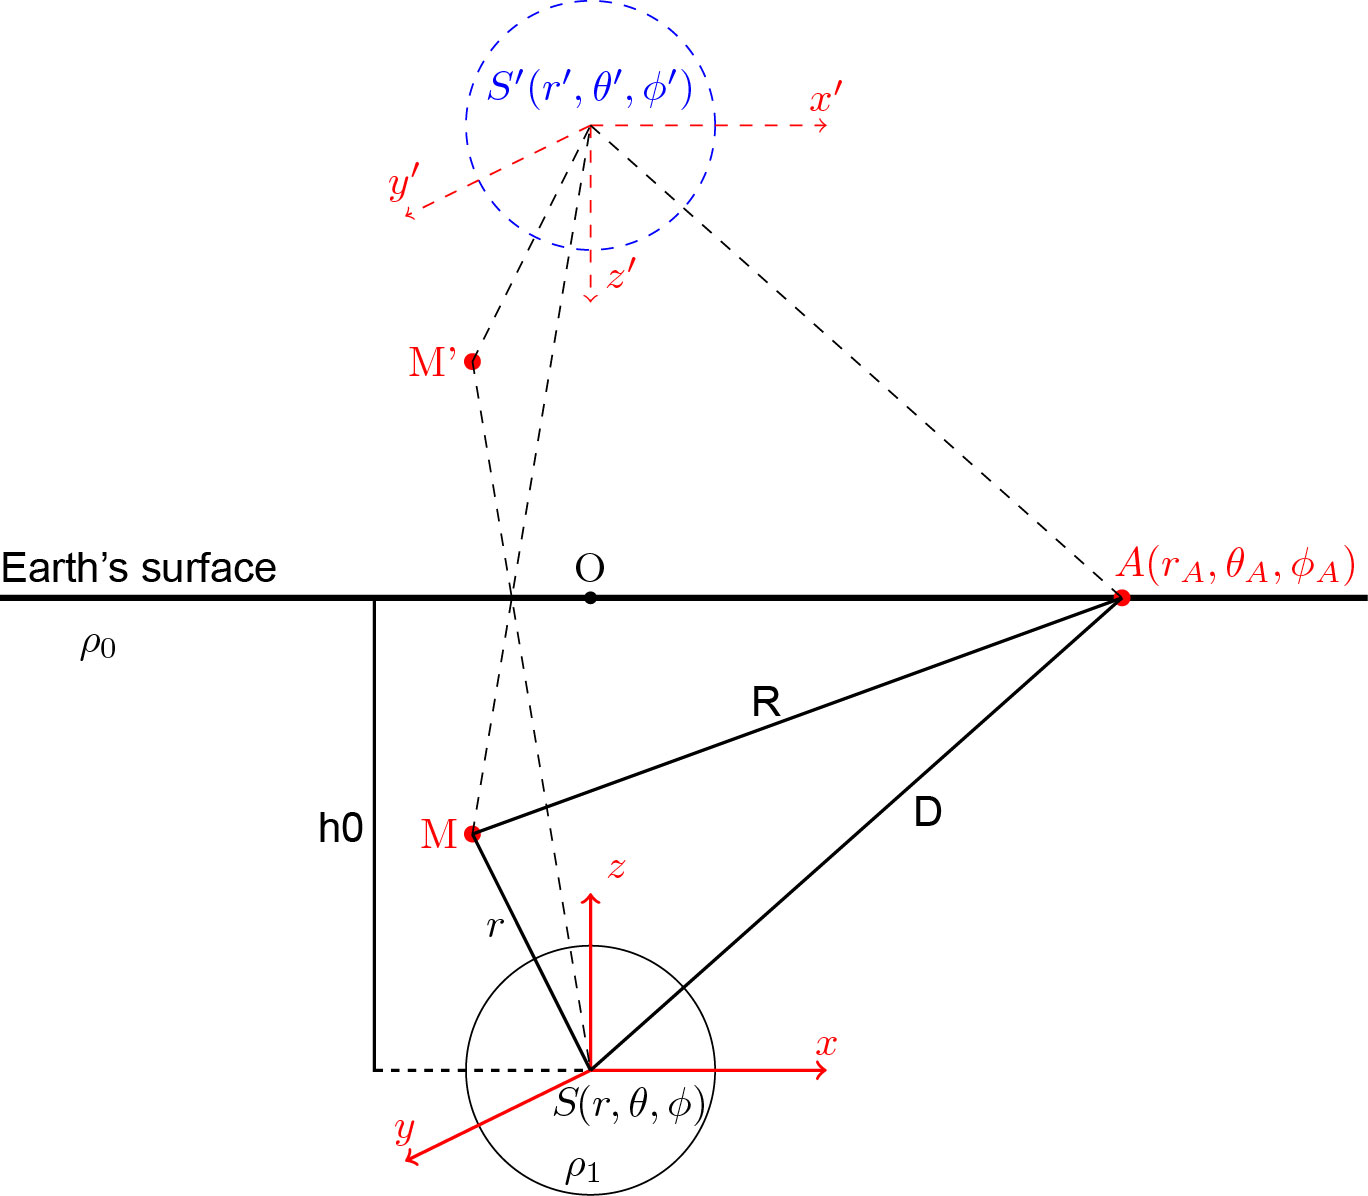
\includegraphics[width=0.7\textwidth]{sketch.jpg}
\caption{Sketch of a spherical body in a uniform earth.}
\label{fig:sketch}
\end{figure}
For convenience, the earth is divided into exterior region 1 and interior region 2 to the sphere.  In a bispherical coordiante system, the total potential $V$ can be expressed as the sum of a primary potential $V_p$, a secondary potential $V_s$ caused by the sphere, and a virtual potential $V_i$ due to the image of the spherical body. The potentials for sites in region 1 and 2 are
\begin{align}
V_1 &= V_p + V_{s1} + V_i \\
V_2 &= V_p + V_{s2} + V_i
\end{align}
In regions free of charge, the potential is governed by the Laplace's equation
% Laplace equation
\begin{equation}\label{eq:laplace_eq}
\frac{\partial}{\partial r}(r^2\frac{\partial V}{\partial r}) + \frac{1}{\sin\theta}\frac{\partial}{\partial\theta}(\sin\theta\frac{\partial V}{\partial\theta}) + \frac{1}{\sin^2\theta}\frac{\partial^2 V}{\partial\phi^2} = 0
\end{equation}
The general solution for potential $V$ can be obtained by applying the method of separation of variables 
\begin{equation}\label{eq:lap_sln}
V = \sum\limits_{n=0}^\infty \sum\limits_{m=0}^n (A_{mn}r^n + B_{mn}r^{-n-1}) \times [C_{mn}\cos(m\phi) + D_{mn}\sin(m\phi)]P_n^m\cos\theta
\end{equation}
Considering the boundary condition at surface of sphere
\begin{subequations}
\begin{align}\label{eq:bcs}
\frac{\partial V_1}{\partial r}|_{r=h_0} = 0 \\
V_1 = V_2 \quad \text{ for } r = r_0 \\
\frac{1}{\rho_1}\frac{\partial V_1}{\partial r} = \frac{1}{\rho_2}\frac{\partial V_2}{\partial r}|_{r=r_0}
\end{align}
\end{subequations}
where $r_0$ is the radius of the sphere. Applying boundary conditions \eqref{eq:bcs} to \eqref{eq:lap_sln}, we obtains 
\begin{align}
V_{s1} &= \sum\limits_{n=0}^\infty(\frac{r_0}{r})^{n+1}\sum\limits_{m=0}^n [A_{mn}\cos(m\phi) + B_{mn}\sin(m\phi)]P_n^m \cos\phi \label{eq:sp1}\\
V_{s2} &=\sum\limits_{n=0}^\infty(\frac{r_0}{r})^{n}\sum\limits_{m=0}^n [C_{mn}\cos(m\phi) + D_{mn}\sin(m\phi)]P_n^m \cos\phi \label{eq:sp2}
\end{align}
where $A_{mn}, B_{mn}, C_{mn}$ and $D_{mn}$ are unknown coefficients. $P_n^m$ is the Legendre function of the first kind. The primary potential may be also expanded in bispherical coordinates as
\begin{equation}\label{eq:primary_p}
\begin{split}
V_p &= \frac{\rho_0I}{4\pi}\sum\limits_{n=0}^\infty\frac{r^n}{D^{n+1}}\{P_n\cos\theta_A P_n\cos\theta + 2\sum\limits_{m=1}^n\frac{(n-m)!}{(n+m)!}[\cos(m\phi_A)\cos(m\phi) \\
&+ \sin(m\phi_A)\sin(m\phi)] \times P_n^m\cos\theta_A P_n^m\cos\theta \}
\end{split}
\end{equation}
when $r > D$, the position of $r$ and $D$ in above equation should be exchanged.  

The virtual potential due to image of the sphere $S'$ is
\begin{equation}\label{eq:virtual_p}
V_i(r,\theta,\phi) = \sum\limits_{n=0}^\infty(\frac{r_0}{r_i})^{n+1}\sum\limits_{m=0}^n [A_{mn}\cos(m\phi_i) + B_{mn}\sin(m\phi_i)]P_n^m\cos\phi_i
\end{equation}
where$(r_i,\theta_i,\phi_i)$ is for spherical coordinate $S'$. Considering the equivalence of potential site $M(r,\theta,\phi)$ in spherical coordinate $S$ with virtual potential site $M'(r_i,\theta_i,\phi_i)$ in coordinate $S'$, we have

\begin{subequations}\label{eq:bi_equal}
\begin{align}
P_n^m(\cos\theta_i)r_i^{-n-1} &= \sum\limits_{k=m}^\infty \frac{(n+k)!}{(n-m)!(m+k)!}\frac{r_i^{\prime	k}}{h_0^{n+k+1}}P_k^m\cos\theta_i^\prime \\
\phi &= \phi_i^\prime
\end{align}
\end{subequations}

Substitute equation \eqref{eq:bi_equal} into equation \eqref{eq:virtual_p}, 
\begin{equation}\label{eq:vpnew}
V_i = \sum\limits_{n=0}^\infty\sum\limits_{m=0}^\infty r_0^{n+1}[A_{mn}\cos(m\phi) + B_{mn}\sin(m\phi)] \times \sum\limits_{k=m}^\infty\frac{(n+k)!}{(n-m)!(m+k)!}\frac{r^k}{h_0^{n+k+1}}P_k^m\cos\phi
\end{equation}

Rearranging equations \eqref{eq:sp1}\eqref{eq:sp2}\eqref{eq:primary_p}\eqref{eq:vpnew}, we have
\begin{align}
V_1 &= \frac{\rho_0 I}{4\pi}\sum\limits_{n=0}^\infty\frac{r^n}{D^{n+1}}L_m(\theta_A,\phi_A,\theta,\phi) + V_i + \sum\limits_{n=0}^\infty(\frac{r_0}{r})^{n+1}Y_m(\theta,\phi) \\
V_2 &= \frac{\rho_0 I}{4\pi}\sum\limits_{n=0}^\infty\frac{r^n}{D^{n+1}}L_m(\theta_A,\phi_A,\theta,\phi) + V_i + \sum\limits_{n=0}^\infty(\frac{r_0}{r})^{n}Y^\prime_m(\theta,\phi)
\end{align}
where
\begin{align}
Y_m(\theta,\phi) &= \sum\limits_{m=0}^\infty[A_{mn}\cos(m\phi)+B_{mn}\sin(m\phi)]P_n^m\cos(\phi) \\
Y_m^\prime(\theta,\phi) &= \sum\limits_{m=0}^\infty[C_{mn}\cos(m\phi)+D_{mn}\sin(m\phi)]P_n^m\cos(\phi) 
\end{align}
and
\begin{equation}
\begin{split}
L_m(\theta_A,\phi_A,\theta,\phi) &= P_n\cos\theta_A P_n\cos\theta + 2\sum\limits_{m=1}^n\frac{(n-m)!}{(n+m)!}[\cos(m\phi_A)\cos(m\phi) + \\
&\sin(m\phi_A)\sin(m\phi)] \times P_n^m\cos\theta_A P_n^m\cos\theta
\end{split}
\end{equation}


 \vspace{0.4cm}



\section{Analytic solution for a buried sphere in a uniform space} 
Extensive studies have been carried out concerning the solution for a buried spherical body in a homogeneous earth due to a point source on the earth's surface. We summarize a general procedure to this problem based on image method. A bispherical coordinate system  is usually used considering the boundary conditions on both the spherical and planar surface. 
Figure \ref{fig:sketch} shows the bispherical system for a conducting sphere with conductivity $\rho_1$ buried in a uniform earth with conductivity $\rho_0$, $A$ is the current point located on the x axis with bispherical coordinate $(r_A,\theta_A,\phi_A)$, here $r_A=D, \theta_A=arcos(h_0/D), \phi_A=\pi$. $D$ is the distance between the current point $A$ and center of buried sphere, $R$ is the distance between $A$ and an arbitrary potential site $M$. 
\begin{figure}[h!]
\centering
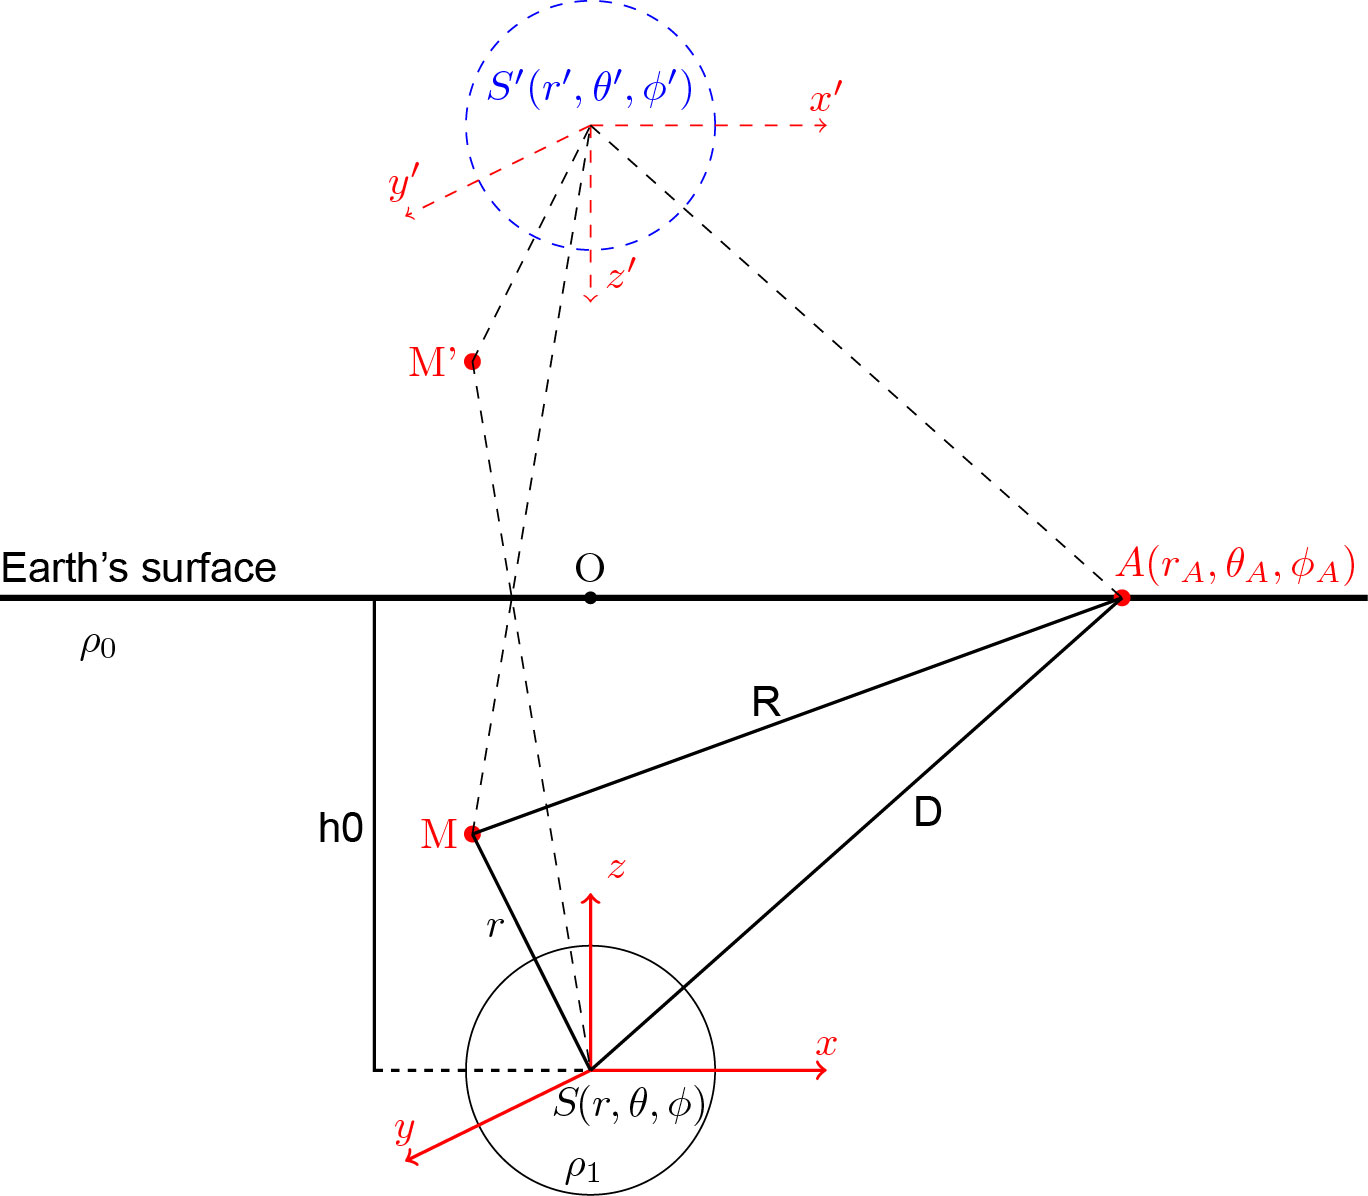
\includegraphics[width=0.7\textwidth]{sketch.jpg}
\caption{Sketch of a spherical body in a uniform earth.}
\label{fig:sketch}
\end{figure}
For convenience, the earth is divided into exterior region 1 and interior region 2 to the sphere.  In a bispherical coordiante system, the total potential $V$ can be expressed as the sum of a primary potential $V_p$, a secondary potential $V_s$ caused by the sphere, and a virtual potential $V_i$ due to the image of the spherical body. The potentials for sites in region 1 and 2 are
\begin{align}
V_1 &= V_p + V_{s1} + V_i \\
V_2 &= V_p + V_{s2} + V_i
\end{align}
In regions free of charge, the potential is governed by the Laplace's equation
% Laplace equation
\begin{equation}\label{eq:laplace_eq}
\frac{\partial}{\partial r}(r^2\frac{\partial V}{\partial r}) + \frac{1}{\sin\theta}\frac{\partial}{\partial\theta}(\sin\theta\frac{\partial V}{\partial\theta}) + \frac{1}{\sin^2\theta}\frac{\partial^2 V}{\partial\phi^2} = 0
\end{equation}
The general solution for potential $V$ can be obtained by applying the method of separation of variables 
\begin{equation}\label{eq:lap_sln}
V = \sum\limits_{n=0}^\infty \sum\limits_{m=0}^n (A_{mn}r^n + B_{mn}r^{-n-1}) \times [C_{mn}\cos(m\phi) + D_{mn}\sin(m\phi)]P_n^m\cos\theta
\end{equation}
Considering the boundary condition at surface of sphere
\begin{subequations}
\begin{align}\label{eq:bcs}
\frac{\partial V_1}{\partial r}|_{r=h_0} = 0 \\
V_1 = V_2 \quad \text{ for } r = r_0 \\
\frac{1}{\rho_1}\frac{\partial V_1}{\partial r} = \frac{1}{\rho_2}\frac{\partial V_2}{\partial r}|_{r=r_0}
\end{align}
\end{subequations}
where $r_0$ is the radius of the sphere. Applying boundary conditions \eqref{eq:bcs} to \eqref{eq:lap_sln}, we obtains 
\begin{align}
V_{s1} &= \sum\limits_{n=0}^\infty(\frac{r_0}{r})^{n+1}\sum\limits_{m=0}^n [A_{mn}\cos(m\phi) + B_{mn}\sin(m\phi)]P_n^m \cos\phi \label{eq:sp1}\\
V_{s2} &=\sum\limits_{n=0}^\infty(\frac{r_0}{r})^{n}\sum\limits_{m=0}^n [C_{mn}\cos(m\phi) + D_{mn}\sin(m\phi)]P_n^m \cos\phi \label{eq:sp2}
\end{align}
where $A_{mn}, B_{mn}, C_{mn}$ and $D_{mn}$ are unknown coefficients. $P_n^m$ is the Legendre function of the first kind. The primary potential may be also expanded in bispherical coordinates as
\begin{equation}\label{eq:primary_p}
\begin{split}
V_p &= \frac{\rho_0I}{4\pi}\sum\limits_{n=0}^\infty\frac{r^n}{D^{n+1}}\{P_n\cos\theta_A P_n\cos\theta + 2\sum\limits_{m=1}^n\frac{(n-m)!}{(n+m)!}[\cos(m\phi_A)\cos(m\phi) \\
&+ \sin(m\phi_A)\sin(m\phi)] \times P_n^m\cos\theta_A P_n^m\cos\theta \}
\end{split}
\end{equation}
when $r > D$, the position of $r$ and $D$ in above equation should be exchanged.  

The virtual potential due to image of the sphere $S'$ is
\begin{equation}\label{eq:virtual_p}
V_i(r,\theta,\phi) = \sum\limits_{n=0}^\infty(\frac{r_0}{r_i})^{n+1}\sum\limits_{m=0}^n [A_{mn}\cos(m\phi_i) + B_{mn}\sin(m\phi_i)]P_n^m\cos\phi_i
\end{equation}
where$(r_i,\theta_i,\phi_i)$ is for spherical coordinate $S'$. Considering the equivalence of potential site $M(r,\theta,\phi)$ in spherical coordinate $S$ with virtual potential site $M'(r_i,\theta_i,\phi_i)$ in coordinate $S'$, we have

\begin{subequations}\label{eq:bi_equal}
\begin{align}
P_n^m(\cos\theta_i)r_i^{-n-1} &= \sum\limits_{k=m}^\infty \frac{(n+k)!}{(n-m)!(m+k)!}\frac{r_i^{\prime	k}}{h_0^{n+k+1}}P_k^m\cos\theta_i^\prime \\
\phi &= \phi_i^\prime
\end{align}
\end{subequations}

Substitute equation \eqref{eq:bi_equal} into equation \eqref{eq:virtual_p}, 
\begin{equation}\label{eq:vpnew}
V_i = \sum\limits_{n=0}^\infty\sum\limits_{m=0}^\infty r_0^{n+1}[A_{mn}\cos(m\phi) + B_{mn}\sin(m\phi)] \times \sum\limits_{k=m}^\infty\frac{(n+k)!}{(n-m)!(m+k)!}\frac{r^k}{h_0^{n+k+1}}P_k^m\cos\phi
\end{equation}

Rearranging equations \eqref{eq:sp1}\eqref{eq:sp2}\eqref{eq:primary_p}\eqref{eq:vpnew}, we have
\begin{align}
V_1 &= \frac{\rho_0 I}{4\pi}\sum\limits_{n=0}^\infty\frac{r^n}{D^{n+1}}L_m(\theta_A,\phi_A,\theta,\phi) + V_i + \sum\limits_{n=0}^\infty(\frac{r_0}{r})^{n+1}Y_m(\theta,\phi) \\
V_2 &= \frac{\rho_0 I}{4\pi}\sum\limits_{n=0}^\infty\frac{r^n}{D^{n+1}}L_m(\theta_A,\phi_A,\theta,\phi) + V_i + \sum\limits_{n=0}^\infty(\frac{r_0}{r})^{n}Y^\prime_m(\theta,\phi)
\end{align}
where
\begin{align}
Y_m(\theta,\phi) &= \sum\limits_{m=0}^\infty[A_{mn}\cos(m\phi)+B_{mn}\sin(m\phi)]P_n^m\cos(\phi) \\
Y_m^\prime(\theta,\phi) &= \sum\limits_{m=0}^\infty[C_{mn}\cos(m\phi)+D_{mn}\sin(m\phi)]P_n^m\cos(\phi) 
\end{align}
and
\begin{equation}
\begin{split}
L_m(\theta_A,\phi_A,\theta,\phi) &= P_n\cos\theta_A P_n\cos\theta + 2\sum\limits_{m=1}^n\frac{(n-m)!}{(n+m)!}[\cos(m\phi_A)\cos(m\phi) + \\
&\sin(m\phi_A)\sin(m\phi)] \times P_n^m\cos\theta_A P_n^m\cos\theta
\end{split}
\end{equation}

\section{DC app for looking at currents, charges etc with a current source at the surface}

\bibliography{refs}
\end{document}